\documentclass[11pt]{article}
\usepackage[margin=1.1in]{geometry}
\usepackage{amsmath,amssymb,amsthm}
\usepackage{booktabs}
\usepackage{graphicx}
\usepackage[round]{natbib}
\usepackage{hyperref}
\hypersetup{hidelinks}
\usepackage{microtype}

\newtheorem{proposition}{Proposition}
\theoremstyle{remark}
\newtheorem{remark}[proposition]{Remark}

\newcommand{\E}{\mathbb{E}}
\newcommand{\I}{\mathrm{I}}
\newcommand{\given}{\,|\,}

\title{A Grammar of Transforms for Probabilistic Forecasting,\\ Nesting Split Conformal Prediction}
\author{Peter Cotton\\\texttt{peter.cotton@microprediction.com}}
\date{August 2026}

\begin{document}
\maketitle

\begin{abstract}
The conformal literature organizes itself around prediction-set constructions. We organize
around transform grammars instead. The fence-post empirical distribution function, smoothed
and composed with the probit, is an invertible online transform, so conformal prediction
becomes one production rule in a grammar of chained transforms. On 701 economic series,
refitting on the transformed stream beats stopping at it on three quarters of the series,
and a likelihood-weighted pool that admits the conformal pattern pays nothing for admitting
it while trimming its worst cases. Which guarantees survive composition depends on position
in the chain, and the operator's value depends on the scoring rule.
\end{abstract}

\section{Introduction}\label{sec:intro}

Split conformal prediction can be written as a chain. Fit a model, take residuals, apply
the fence-post empirical transform
\begin{equation}\label{eq:fencepost}
E_n(r) \;=\; \frac{1 + \#\{i \le n : R_i \le r\}}{n+1},
\end{equation}
and map the resulting rank back through the model to a prediction set
\citep{vovk2005algorithmic,lei2018distribution}. The value of \eqref{eq:fencepost} at a
new point is a conformal p-value, and the map itself is the unrandomized conformal
predictive distribution of \citet{vovk2019nonparametric}. We call it the fence-post
transform, after the two $+1$ corrections. The literature treats this chain as a
construction to be studied whole, and its many variants, normalized, Mondrian, quantile,
distributional, and temporal
\citep{bostrom2021mondrian,romano2019conformalized,chernozhukov2021distributional,gibbs2021adaptive,auer2023hopcpt},
as separate constructions. We propose a different organization. The fence-post transform is
one operator. The chain is one production rule in a grammar of composable transforms. The
interesting question is then not which conformal method to choose but which sequence of
transforms minimizes the forecaster's scoring rule.

This reorganization has content because the fence-post operator composes. Once smoothed,
$E_n$ is an invertible change of variables with a density, and its probit composition
$z = \Phi^{-1}(E_n(r))$ maps exchangeable residuals to approximately standard Gaussian
coordinates. Nothing obliges a forecaster to stop there. One can fit further structure on
the Gaussianized stream, transform again, and continue, exactly as one does with any other
member of the transform library. Conformal calibration stops at the transform. The grammar
keeps going.

Two testable claims follow. The first is that the operator has interior value: refitting on
the Gaussianized stream should beat stopping at it whenever residual structure remains. The
second is that nesting protects: a likelihood-weighted pool over chains that includes the
conformal pattern should never pay materially for admitting it, because the pool reallocates
weight away from the pattern on series where it is a bad choice. We confirm both on 701
economic series and quantify a third finding we did not anticipate: the operator's value
depends on the scoring rule for a structural reason, not an implementation one.

A companion paper prices what a fixed representation choice costs
\citep{cotton2026gap}. Under logarithmic loss the irreducible cost of pooling residuals in
given coordinates is a mutual information, the conformal information gap, and the companion
measures it on the same corpus. The present paper is the constructive complement. If a fixed
conformal pattern can be a bad choice with a quantifiable price, the remedy is not a better
fixed choice. It is a grammar in which the choice is made by the scoring rule, online,
per series.

\section{The fence-post transform as an operator}\label{sec:operator}

We work with online univariate transforms in the sense of the \texttt{skaters} library,
described at length in a methods paper \citep{cotton_skaters} and briefly in a software
paper \citep{cotton_skaters_joss}. A transform is a pair of functions. The forward function consumes
one observation and its own past state and emits a transformed observation. The inverse
function maps predictive distributions in the transformed space back to the original space.
Conditional on its own past state, the forward map is an invertible change of variables in
the current observation, so predictive densities push back exactly, Jacobians included.

The raw fence-post map \eqref{eq:fencepost} is a step function. It has no density and no
inverse, so it is not a transform in this sense. The minimal repair is interpolation. Let
$y_{(1)} \le \dots \le y_{(n)}$ be the past observations, place knots at a bounded number of
order statistics with fence-post probabilities $p_{(i)} = (i+1)/(n+1)$, set
$z_{(i)} = \Phi^{-1}(p_{(i)})$, and interpolate the pairs $(y_{(i)}, z_{(i)})$ piecewise
linearly. We call the resulting operator \emph{gaussianize}. Beyond the edge knots the map
extends linearly in $(y, z)$ coordinates, and linearity in the probit coordinate is a
Gaussian tail in the observable, with scale set by the spacing of the extreme quantiles.
Tail mass is unobservable, so any usable version of the operator carries a tail assumption,
and this is the mildest one consistent with the coordinates. A kernel-smoothed variant
replaces the empirical distribution function with a Gaussian-kernel estimate at Silverman
bandwidth, represented by a monotone $C^1$ cubic through the same knots, and we use it in
Section~\ref{sec:smooth} to test whether smoothness matters.

Two guards complete the definition, and both were forced by data rather than taste. First,
every knot-segment slope is capped at twenty times the interquartile slope. An upstream
variance collapse can plant a many-sigma outlier as an edge knot, and an uncapped edge
segment then hands the inverse map an explosive extrapolation slope. The cap is an explicit
assumption: tail scale at most a fixed multiple of the central scale. Second, the forward
output is clamped to $|z| \le 8$. No fence-post rank exceeds probability $n/(n+1)$, and
$\Phi^{-1}(n/(n+1)) < 8$ for any feasible $n$, so the clamp only removes values the
empirical map itself could never produce. It exists because downstream learners have
expanding memory. In one series in our corpus a degenerate warmup emitted a single
transformed value near $8000$, and the downstream Welford variance and recursive
least-squares state never forgot it, inflating that series' loss by four orders of
magnitude. Composability is not free. An operator that is harmless as a terminal step can
poison downstream learners through one bad emission, and the operator's definition has to
prevent this, not the caller.

Before enough observations accumulate, the operator standardizes by expanding moments,
which is the $n \to 0$ limit of the empirical map. After the warmup the knots are rebuilt
from a bounded quantile sketch each step, so memory and per-step cost do not grow with the
series.

\section{What composition preserves}\label{sec:typing}

Each operator in a grammar carries properties. It may be monotone, invertible,
density-carrying, exchangeability-preserving, or finite-sample calibrated. Composition preserves some and
destroys others, and the pattern is positional. We record the three facts that organize our
experiments.

\begin{proposition}[Fence-post uniformity]\label{prop:uniform}
Let $R_1, \dots, R_{n+1}$ be exchangeable and almost surely distinct. Then
$E_n(R_{n+1})$ is uniform on $\{1/(n+1), \dots, (n+1)/(n+1)\}$. In particular,
$\Pr\{E_n(R_{n+1}) \le k/(n+1)\} = k/(n+1)$ for $k = 1, \dots, n+1$.
\end{proposition}

\begin{proof}
By exchangeability every ordering of $R_1, \dots, R_{n+1}$ is equally likely, and by
almost-sure distinctness the rank of $R_{n+1}$ among the $n+1$ values is uniform on
$\{1, \dots, n+1\}$. The map \eqref{eq:fencepost} evaluated at $R_{n+1}$ equals the rank
divided by $n+1$.
\end{proof}

This is the standard conformal fact \citep{vovk2005algorithmic} stated as a property of the
operator's output. It is what makes the operator worth admitting to a grammar at all: it
converts exchangeable inputs into finite-sample calibrated pseudo-uniforms, and after the
probit, into pseudo-Gaussians.

The second fact is that this guarantee is positional. Proposition~\ref{prop:uniform}
concerns the operator's immediate output. If a downstream model is fitted on
$z_1, \dots, z_t$ and its parameters enter later forecasts, the composed system's forecast
at time $t+1$ depends on the ordering of the past stream, and the exchangeability that
delivered uniformity no longer applies to the composed output. The calibration certificate
attaches to a position in the chain, not to the chain. This is not a defect. It is the
familiar price of fitting, and the reason the companion paper's ledger separates
representation, model-form, and estimation cost \citep{cotton2026gap}. But it means the
grammar has a typing discipline: an operator's guarantee names the position at which it
holds, and claims about the composed system need their own arguments.

The third fact prices the choice of coordinates. The companion paper's transform-pooling
theorem states that pooling residuals after an invertible state-dependent change of
coordinates $\phi_X$ has irreducible log-score gap $\I(\phi_X(R); X)$: the Jacobians of the
transform cancel, and only the coordinates' ability to remove conditional heterogeneity
matters \citep{cotton2026gap}. The gaussianize operator is a data-dependent monotone map,
measurable with respect to its own past state, and piecewise $C^1$, so conditional on the
state the theorem's hypotheses hold. The grammar view adds only this: since operators
compose, the coordinates in which one pools are themselves a product of the chain, and the
gap is a property of the whole chain up to the pooling point.

The classical antecedent of the chain view is the Rosenblatt transformation
\citep{rosenblatt1952remarks}, which Gaussianizes by composing conditional distribution
functions. Normalizing flows are its learned, offline descendants: compositions of
invertible maps trained by log score \citep{papamakarios2021normalizing}. The grammar
studied here is the online, exchangeability-aware member of the family, and the fence-post
operator is what distinguishes it: a rank-based link whose output carries a finite-sample
guarantee at its position.

\section{Measurements}\label{sec:experiments}

\subsection{Design}\label{sec:design}

The corpus, scoring conventions, and evaluation protocol follow the companion paper
\citep{cotton2026gap}. We use 701 FRED change series with at least 600 observations and
repeat fraction below five percent. Every forecaster runs prequentially: at each time it
issues a one-step predictive density from data strictly before that time, then sees the
observation and updates. Scoring starts after a burn-in of 300 observations. The log score
is exact: each predictive is mixed with weight $0.01$ toward an expanding-window Gaussian
reference, so no clipping or flooring enters the reported nats. CRPS is computed in closed
form from the Gaussian-mixture predictive. Per-series CRPS is normalized by the location
baseline defined next, so scales are comparable across series.

Six single chains and three pools are compared. All chains end in a Gaussian leaf with
online variance, and all transforms update online.

\begin{center}
\small
\begin{tabular}{ll}
\toprule
config & chain \\
\midrule
A & location (EMA) $\to$ leaf \\
B & location $\to$ scale (EWMA standardize) $\to$ leaf \\
C & location $\to$ gaussianize $\to$ leaf \quad (raw conformal pattern) \\
D & location $\to$ scale $\to$ gaussianize $\to$ leaf \quad (normalized pattern) \\
E & location $\to$ scale $\to$ gaussianize $\to$ AR(1) $\to$ leaf \quad (refit through) \\
F & location $\to$ scale $\to$ AR(1) $\to$ leaf \quad (same refit, no gaussianize) \\
G & likelihood-weighted pool over $\{$leaf, A, B, C, D, E, F$\}$ \\
H & the same pool without the gaussianize chains \\
I & the pool of G with kernel-smoothed gaussianize \\
\bottomrule
\end{tabular}
\end{center}

Configs C and D are the conformal production rule written as a chain: transform, apply the
fence-post empirical map, stop, and read the predictive off the inverse. Config E continues
through the operator. The pools use the same likelihood-weighted online ensembling as the
companion paper's forecaster, with a complexity penalty by chain depth.
Figure~\ref{fig:duels} summarizes the comparisons behind the paper's three findings.

\begin{figure}[t]
\centering
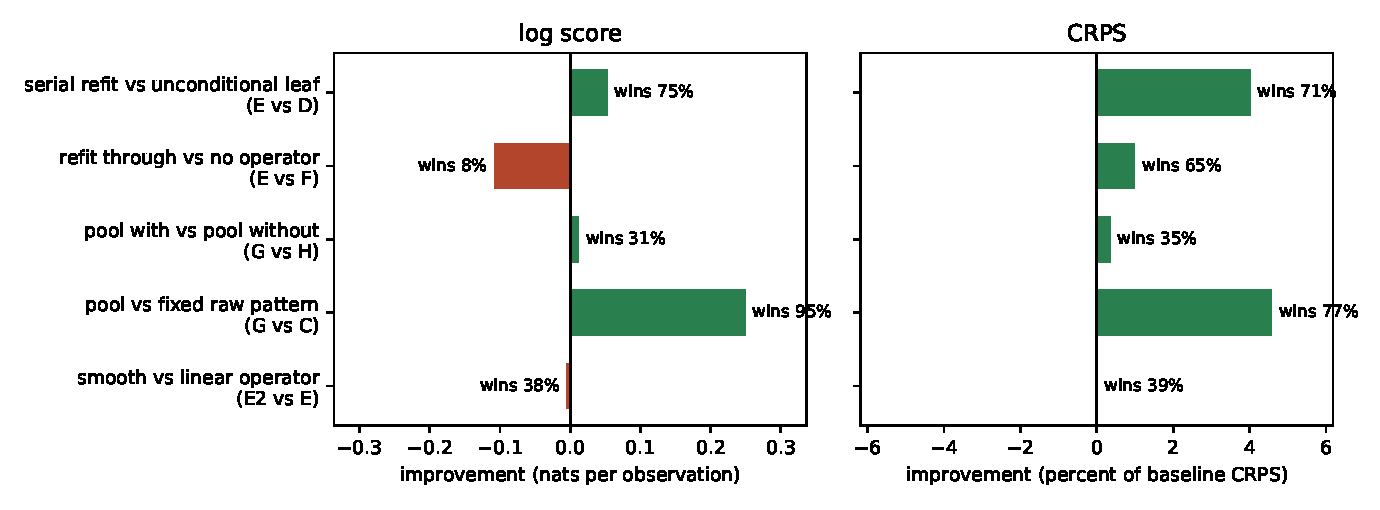
\includegraphics[width=\textwidth]{fig_grammar.pdf}
\caption{The five comparisons behind the three findings, on 701 series under both scoring
rules. Bars to the right favor the first-named config. Log score improvement is in nats per
observation. CRPS improvement is in percent of the location-baseline CRPS. Win rates are
per-series.}\label{fig:duels}
\end{figure}

\subsection{The operator has interior value}\label{sec:interior}

Refitting on the Gaussianized stream beats stopping at it. Config E improves on config D by
$0.053$ nats per observation, winning on $75$ percent of series, and by $4.0$ percent of
baseline CRPS, winning on $71$ percent. The conformal pattern's stopping point is not where
the predictive value stops.

A synthetic experiment shows the mechanism in isolation. Let $z_t = 0.8 z_{t-1} +
\varepsilon_t$ and observe $y_t = \mathrm{sign}(z_t) |z_t|^{1.5}$, a monotone warp of an
AR(1), so the serial structure is visible only in the Gaussianized coordinates. Stopping at
gaussianize scores $-1.56$ nats and $0.62$ CRPS. Refitting AR(1) through it scores $-1.07$
and $0.41$, beating both the stop and the same AR chain without the operator ($-1.16$,
$0.42$). When structure lives in the empirical map's coordinates, the operator is the only
way to reach it, and it must be passed through, not stopped at.

On the real corpus the comparison with config F is sharper and score-dependent. Under CRPS
the operator helps: E beats F on $65$ percent of series, and E is the best single chain in
the study at $0.911$ of baseline. Under the log score the operator costs $0.108$ nats
against F and wins only $8$ percent of series. We return to this in
Section~\ref{sec:smooth}, because the natural suspicion, that the piecewise-linear density
is to blame, turns out to be wrong.

\subsection{Nesting prevents a bad choice}\label{sec:nesting}

The raw conformal pattern C is a reasonable forecaster on this corpus, better than the
location baseline on average under both scores. It is also, on a minority of series, a bad
choice. The pool G that admits the conformal chains beats the fixed pattern C on $95$
percent of series by log score, by $0.249$ nats on average. On the twenty series where C is
worst, with relative CRPS $1.020$, the pool sits at $0.843$ on the same series. The pool
walks away from the production rule where it underperforms.

Admitting the pattern costs nothing. The pools with and without the gaussianize chains
differ by $0.012$ nats and $0.4$ percent of baseline CRPS, with the nesting pool ahead on
both means. This is the practical content of the grammar view. A fixed conformal method is
a commitment, and the companion paper prices what the commitment can cost. A grammar that
contains the method as one rule converts the commitment into a weighted vote, and the vote
is revised online by the scoring rule. Nesting does not avert disasters on this corpus,
because the guarded operator does not produce disasters. It trims the bad tail, for free.

\subsection{Smoothness is not the tax}\label{sec:smooth}

The log-score cost of the operator invites an implementation explanation: the
piecewise-linear empirical map has a piecewise-constant density, and the log score punishes
kinks. The kernel-smoothed $C^1$ variant tests this directly, replacing the interpolated
empirical distribution function with a smooth kernel estimate while changing nothing else.
The explanation fails. The smooth variant tracks the linear one within $0.012$ nats and
$0.2$ percent of baseline CRPS in every position, and against config F it costs $0.113$ nats where
the linear variant cost $0.108$. Smoothness is not the tax.

The tax is structural, and it is the same structure the companion paper measured for
terminal empirical pooling. An empirical map's resolution is bounded by its ranks, and its
tails are an assumption, and the log score is exactly the score that pays for resolution
and tails. Under CRPS, which pays for calibrated quantiles, the operator earns its place in
the chain. Under the log score a fitted parametric leaf on the same stream is worth more.
The value of the fence-post operator, like the value of residual pooling in the companion
paper, depends jointly on the coordinates, the estimator, and the scoring rule. The grammar
does not remove this dependence. It locates it: the scoring rule chooses among chains, and
the operator is a candidate, not a default.

The probit is likewise a choice, not the point. Composing the operator with any further
fixed invertible link leaves the representation content unchanged, since mutual information
is invariant under invertible maps, so the transform-pooling theorem makes the link
representation-irrelevant. What remains is model form. On a 120-series holdout check, a
logistic link in place of the probit shifts results by hundredths of a nat under both
scores, and the shift consistently favors the logistic: the Gaussian leaf pushed through
the heavier-tailed link implies a heavier-tailed predictive, which fits real standardized
residuals slightly better. The link is a small tail-shape knob, and the theorem says it can
be nothing more.

\section{One family}\label{sec:family}

The grammar view collapses a scattered vocabulary. Platt scaling
\citep{platt1999probabilistic}, isotonic calibration \citep{zadrozny2002transforming},
temperature scaling \citep{guo2017calibration}, quantile recalibration
\citep{kuleshov2018accurate}, conformal predictive systems \citep{vovk2019nonparametric},
and distributional conformal prediction \citep{chernozhukov2021distributional} are all
monotone maps applied to a model's output coordinate, differing in what they fit, what they
guarantee, and where in the chain they sit. The forecasting literature's
calibration-sharpness tradition \citep{gneiting2007probabilistic,gneiting2007strictly}
supplies the objective that orders them. In the grammar they are not competing philosophies.
They are operators with types, and a pool over chains can hold several at once.

Conformal prediction keeps a distinguished place in this family. The fence-post operator is the member whose output carries a
finite-sample, distribution-free guarantee at its position in the chain
(Proposition~\ref{prop:uniform}). No fitted recalibration offers that. The grammar view
does not diminish the guarantee. It names what the guarantee attaches to, and it frees the
forecaster to keep transforming afterward.

\section{Conclusion}\label{sec:conclusion}

Conformal prediction is one production rule in a grammar of composable transforms: model,
residual, fence-post empirical map, inverse. Smoothed, the fence-post map is an ordinary
invertible online transform, and the rule's distinguishing stop, quoting the empirical law
where it stands, becomes a choice the scoring rule can overrule. On 701 economic series,
continuing through the operator beats stopping at it on three quarters of the series, a
pool that admits the pattern pays nothing and trims its worst cases, and the operator's
remaining cost under the log score is structural, the resolution and tail price of any
empirical map, not a smoothness artifact.

The typing question is the theory this view opens. An operator's guarantee attaches to a position in a chain. Which properties survive
composition is a discipline we have only begun here, with one operator and three facts,
and the rest of the table is open.

\bibliographystyle{plainnat}
\bibliography{references}
\end{document}
